\section{Simulation}
\label{sec:simulation}

\begin{figure*}[ht]
	%{0.45\textwidth}
	\centering
	%  \resizebox{\linewidth}{!}{
	\begin{adjustbox}{max size={\textwidth}}
		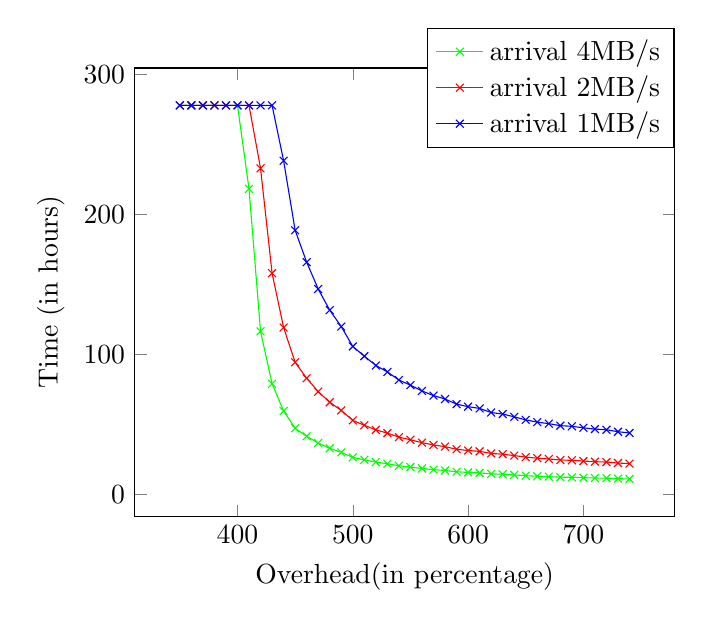
\begin{tikzpicture}
		\begin{axis}[
		%xmode=log,
		legend style={at={(1,1.09)},anchor=north east,legend columns=1},
		xlabel=Overhead(in percentage),
		ylabel=Time (in hours)]
		\addplot[color=green,mark=x] coordinates {
			(350,277.7778028)
			(360,277.7778306)
			(370,277.7777806)
			(380,277.7777806)
			(390,277.777875)
			(400,277.7777972)
			(410,218.0984611)
			(420,116.3991028)
			(430,78.9657)
			(440,59.55381111)
			(450,47.147775)
			(460,41.446375)
			(470,36.65794167)
			(480,32.87560278)
			(490,29.95016111)
			(500,26.40129444)
			(510,24.66028333)
			(520,23.00362222)
			(530,21.85588056)
			(540,20.40405)
			(550,19.48659444)
			(560,18.45943611)
			(570,17.63081111)
			(580,17.01690833)
			(590,16.09901389)
			(600,15.65028056)
			(610,15.33356944)
			(620,14.601075)
			(630,14.32908611)
			(640,13.83495833)
			(650,13.29390556)
			(660,12.88229722)
			(670,12.61861944)
			(680,12.25779722)
			(690,12.14353889)
			(700,11.8762)
			(710,11.64855)
			(720,11.52348611)
			(730,11.17581111)
			(740,10.95483889)
		};
		\addlegendentry{arrival 4MB/s}
		\addplot[color=red,mark=x] coordinates {
			(350,277.7778361)
			(360,277.7777917)
			(370,277.7778389)
			(380,277.7778222)
			(390,277.7777806)
			(400,277.7778056)
			(410,277.7777778)
			(420,232.7982083)
			(430,157.9314)
			(440,119.1076194)
			(450,94.29555)
			(460,82.89275)
			(470,73.31588611)
			(480,65.75120278)
			(490,59.90032222)
			(500,52.80259167)
			(510,49.32056944)
			(520,46.00724722)
			(530,43.71176389)
			(540,40.80809722)
			(550,38.97319167)
			(560,36.91887222)
			(570,35.26162222)
			(580,34.03381667)
			(590,32.19803056)
			(600,31.30056389)
			(610,30.66714167)
			(620,29.20215)
			(630,28.65817222)
			(640,27.66991667)
			(650,26.58781389)
			(660,25.76459444)
			(670,25.23723611)
			(680,24.51559722)
			(690,24.28707778)
			(700,23.75239722)
			(710,23.2971)
			(720,23.046975)
			(730,22.35162222)
			(740,21.909675)
		};
		\addlegendentry{arrival 2MB/s}				
		\addplot[color=blue,mark=x] coordinates {
			(350,277.7778694)
			(360,277.7777944)
			(370,277.7779611)
			(380,277.7778389)
			(390,277.7777889)
			(400,277.7779139)
			(410,277.7778056)
			(420,277.7778167)
			(430,277.777875)
			(440,238.2152389)
			(450,188.5911)
			(460,165.7855028)
			(470,146.6317694)
			(480,131.5024056)
			(490,119.8006444)
			(500,105.6051806)
			(510,98.64113611)
			(520,92.01449444)
			(530,87.42352778)
			(540,81.61619722)
			(550,77.94638056)
			(560,73.83774444)
			(570,70.52324444)
			(580,68.06763333)
			(590,64.39605833)
			(600,62.60112778)
			(610,61.33428056)
			(620,58.40430278)
			(630,57.31634722)
			(640,55.33983056)
			(650,53.175625)
			(660,51.52919167)
			(670,50.474475)
			(680,49.03119167)
			(690,48.57415278)
			(700,47.50479722)
			(710,46.59420278)
			(720,46.09394722)
			(730,44.70324722)
			(740,43.81935)
		};
		\addlegendentry{arrival 1MB/s}				
		\end{axis}
		\end{tikzpicture}
	\end{adjustbox}
	%  }
	\captionsetup{justification=centering}
	\caption{Simulation results for debug-window sizes with gradually increasing the overhead in service processing times. The buffer is kept at a constant 64GB.}
	\label{fig:debugSim}
\end{figure*}


We ran a series of simulation with \textit{poisson} distribution of arrival and service times and modified buffer sizes for each set of runs.
As discussed earlier, there are three parameters which can impact the time period of the debug-window: (1) arrival rate ($\lambda$), (2) service processing time ($\mu$), and (3) Buffer Size.

In our simulations , we kept a constant buffer size of 64GB, and iteratively increased the overhead of instrumentation, thereby decreasing the service processing time.
Each series(set of experiment), starts with an arrival rate approximately 5 times less than the service processing time. 
This means that at 400\% overhead, the system would be running at full capacity.
Each simulation instance was run for 1000000 seconds or 277.7 hours.
We gradually increased the instrumentation by 10~\% each time, and observed the \textit{hitting-time} of the buffer (time it takes for the buffer to overflow for the first time).
As shown in Figure~\ref{fig:debugSim}, there is no buffer overflow in any of the experiments till the overhead reaches around 420-470\%, beyond this the debug-window decreases exponentially

In the first set of simulations, we kept a constant inter-arrival rate ,service time, and increased the buffer iteratively. 
The experiment was repeated for several different service time, and each was plotted as a different series.
The results have been shown in Figure~\ref{fig:sim1}.

In the next set of simulations, we kept a constant inter-arrival rate, buffer, and increased service time with 10~\% overhead.
The experiment was repeated for several different buffer sizes, and each was plotted as a separate series.
The results have been shown in Figure~\ref{fig:sim2}

Based on our experiments we were able to verify that as long as the average service processing time is faster or comparable to the arrival rate (even if arrival rate is slightly faster), the buffer is unlikely to overflow, or have an extremely large debug-window (several hours).
However, this \textit{debug-window} decreases sharply as the service processing time increases, and it is more than the arrival rate. 



\iffalse
Based on equation~\ref{eq:hitting}, we ran a number of simulations to calculate theoretical debug-window sizes based on various resource constraints. 
As discussed earlier, the debug-window primarily depends on 3 parameters, firstly the incoming rate of requests, the overhead in the debug container, and the size of the buffer.
In our simulations shown in Table~\ref{tab:simulation}, we ran multiple iterations with randomized input parameters within pre-defined ranges. 
We assume, an incoming requests to follow a poisson distribution,  with the rate between 30-40 Mbps, we assume a buffer size between 2GB-8GB, and an overhead between 2x-4x. 

Our results indicate that despite heavy overhead with a decent sized buffer, developers can get debug window sizes of more than an hour. 
 
\begin{table}[]
\centering
\begin{tabular}{|r|r|r|r|}
\hline
\multicolumn{1}{|c|}{{\bf \begin{tabular}[c]{@{}c@{}}Request \\ Rate(MB/s)\end{tabular}}} & \multicolumn{1}{c|}{{\bf \begin{tabular}[c]{@{}c@{}}Overhead \\ (2-4x)\end{tabular}}} & \multicolumn{1}{c|}{{\bf \begin{tabular}[c]{@{}c@{}}Buffer \\ Size(MB)\end{tabular}}} & \multicolumn{1}{c|}{{\bf \begin{tabular}[c]{@{}c@{}}Debug-\\ Window (mins)\end{tabular}}} \\ \hline
35 & 3 & 2113 & 17.60869048 \\ \hline
30 & 2 & 2166 & 36.1 \\ \hline
34 & 2 & 2641 & 44.01666667 \\ \hline
33 & 4 & 2728 & 15.15600449 \\ \hline
36 & 4 & 2911 & 16.17263374 \\ \hline
36 & 3 & 3042 & 25.35034722 \\ \hline
31 & 2 & 3201 & 53.35 \\ \hline
39 & 3 & 3274 & 27.28365385 \\ \hline
33 & 3 & 3419 & 28.49204545 \\ \hline
30 & 4 & 3491 & 19.39493827 \\ \hline
39 & 3 & 3516 & 29.30032051 \\ \hline
30 & 3 & 3626 & 30.21708333 \\ \hline
37 & 4 & 4209 & 23.38373373 \\ \hline
36 & 2 & 4242 & 70.7 \\ \hline
34 & 4 & 4472 & 24.84488017 \\ \hline
30 & 4 & 4580 & 25.44493827 \\ \hline
40 & 2 & 4619 & 76.98333333 \\ \hline
40 & 4 & 4883 & 27.12814815 \\ \hline
34 & 3 & 4891 & 40.75870098 \\ \hline
35 & 4 & 4961 & 27.56153439 \\ \hline
36 & 4 & 4982 & 27.6781893 \\ \hline
39 & 4 & 5303 & 29.46149098 \\ \hline
34 & 3 & 5754 & 47.95036765 \\ \hline
31 & 2 & 5994 & 99.9 \\ \hline
35 & 2 & 6060 & 101 \\ \hline
30 & 4 & 6253 & 34.73938272 \\ \hline
31 & 2 & 6898 & 114.9666667 \\ \hline
35 & 4 & 6938 & 38.54486772 \\ \hline
36 & 4 & 6972 & 38.73374486 \\ \hline
34 & 4 & 7231 & 40.17265795 \\ \hline
38 & 2 & 7241 & 120.6833333 \\ \hline
36 & 4 & 7267 & 40.37263374 \\ \hline
33 & 2 & 7374 & 122.9 \\ \hline
36 & 4 & 7404 & 41.13374486 \\ \hline
35 & 3 & 7664 & 63.86702381 \\ \hline
33 & 3 & 7748 & 64.56704545 \\ \hline
35 & 2 & 7770 & 129.5 \\ \hline
33 & 3 & 7868 & 65.56704545 \\ \hline
33 & 4 & 7967 & 44.26156004 \\ \hline
38 & 3 & 7968 & 66.40032895 \\ \hline
\end{tabular}
\caption{Simulation Results for Debug-Window}
\label{tab:simulation}
\end{table}
\fi	